% Grammarly'd
\section{Initial Greedy Algorithm}
\label[section]{sec:failedalg}
\begin{leftbar}
    \noindent
    \textbf{Motivation:} 
    Since time coherence only exists as a connection between one set of streamlines to another,
    we start by creating an algorithm capable of generating such streamlines.
    We then use this algorithm to generate sets of streamlines for time frames without
    time coherence as a negative example and to illustrate the effects of its absence.
    Initially, we developed the algorithm for the 2D case; \Cref{sec:3D} contains the extension to 3D.
\end{leftbar}
\noindent
Our first approach uses two operations, streamline traversal and seed filtering,
which it executes round-robin until there is no more room for new streamlines.
The result is a space-filling set of streamlines with an even spacing in 2D and 3D vector fields.

We use two essential parameters to control image generation.
The first one, $d_s$, is the neighbor search distance,
which controls the distance from the current streamline where new streamlines start,
allowing us to fill the whole space.
In order to add longer streamlines while guaranteeing even spacing,
we introduce a second parameter, $d_c$, which is the neighbor cutoff distance.

As soon as a streamline comes within this distance to another streamline, it is terminated.
The typical range for $d_c$ is $0.5\,d_s \leq d_c \leq 0.75\,d_s$.
Making $d_c$ smaller than $0.5\,d_s$ allows streamlines to get very close,
introducing visual clutter and a crowded appearance.
At values $\geq0.75\,d_s$, many streamlines are very short in forward or backward time due to the proximity of $d_s$ and $d_c$,
causing most of them to be removed immediately.
\subsection{Two-Dimensional Implementation}
\begin{figure}[ht]
    \centering
    \begin{subfigure}[b]{0.3\textwidth}
        \centering
        \begin{tikzpicture}[domain=0:4, scale=.8]
    \draw[very thin,color=gray] (-0.1,-0.1) grid (3.9,3.9);

    \draw[->] (-0.2,0) -- (4.2,0) node[right] {$x$};
    \draw[->] (0,-0.2) -- (0,4.2) node[above] {$y$};

    \draw[dotted, thick]                       (1.5,0) -- (1.5,1) -- (1.73,1.87) -- (2.3,2.78) -- (3,3.4) -- (4,4);
    \draw plot[only marks, mark=x] coordinates{(1.5,0)               (1.73,1.87)    (2.3,2.78)    (3,3.4)};
    
    \draw[red] plot[only marks, mark=*] coordinates{      (1.5,1)};
\end{tikzpicture}

        \caption*{(a)}
    \end{subfigure}
    \begin{subfigure}[b]{0.3\textwidth}
        \centering
        \begin{tikzpicture}[domain=0:4, scale=.8]
    \draw[very thin,color=gray] (-0.1,-0.1) grid (3.9,3.9);
    
    \draw[->] (-0.2,0) -- (4.2,0) node[right] {$x$};
    \draw[->] (0,-0.2) -- (0,4.2) node[above] {$y$};
    
    \draw[dotted, thick]                       (1.5,0) -- (1.5,1) -- (1.73,1.87) -- (2.3,2.78) -- (3,3.4) -- (4,4);
    \draw plot[only marks, mark=x] coordinates{(1.5,0)               (1.73,1.87)    (2.3,2.78)    (3,3.4)};
    
    \draw[black ,arrows={Circle[green]-Circle[green]}] (0.6,  1.1 ) -- (2.4 , 0.9 );
    \draw[black ,arrows={Circle[green]-Circle[green]}] (0.91, 2.2 ) -- (2.59, 1.53);
    \draw[black ,arrows={Circle[green]-Circle[green]}] (1.57, 3.33) -- (3.05, 2.2 );
    \draw[black ,arrows={Circle[green]-Circle[green]}] (2.5 , 4   ) -- (3.55, 2.75);

    \draw[red] plot[only marks, mark=*] coordinates{(1.5,1)};
\end{tikzpicture}

        \caption*{(b)}
    \end{subfigure}
    \begin{subfigure}[b]{0.3\textwidth}
        \centering
        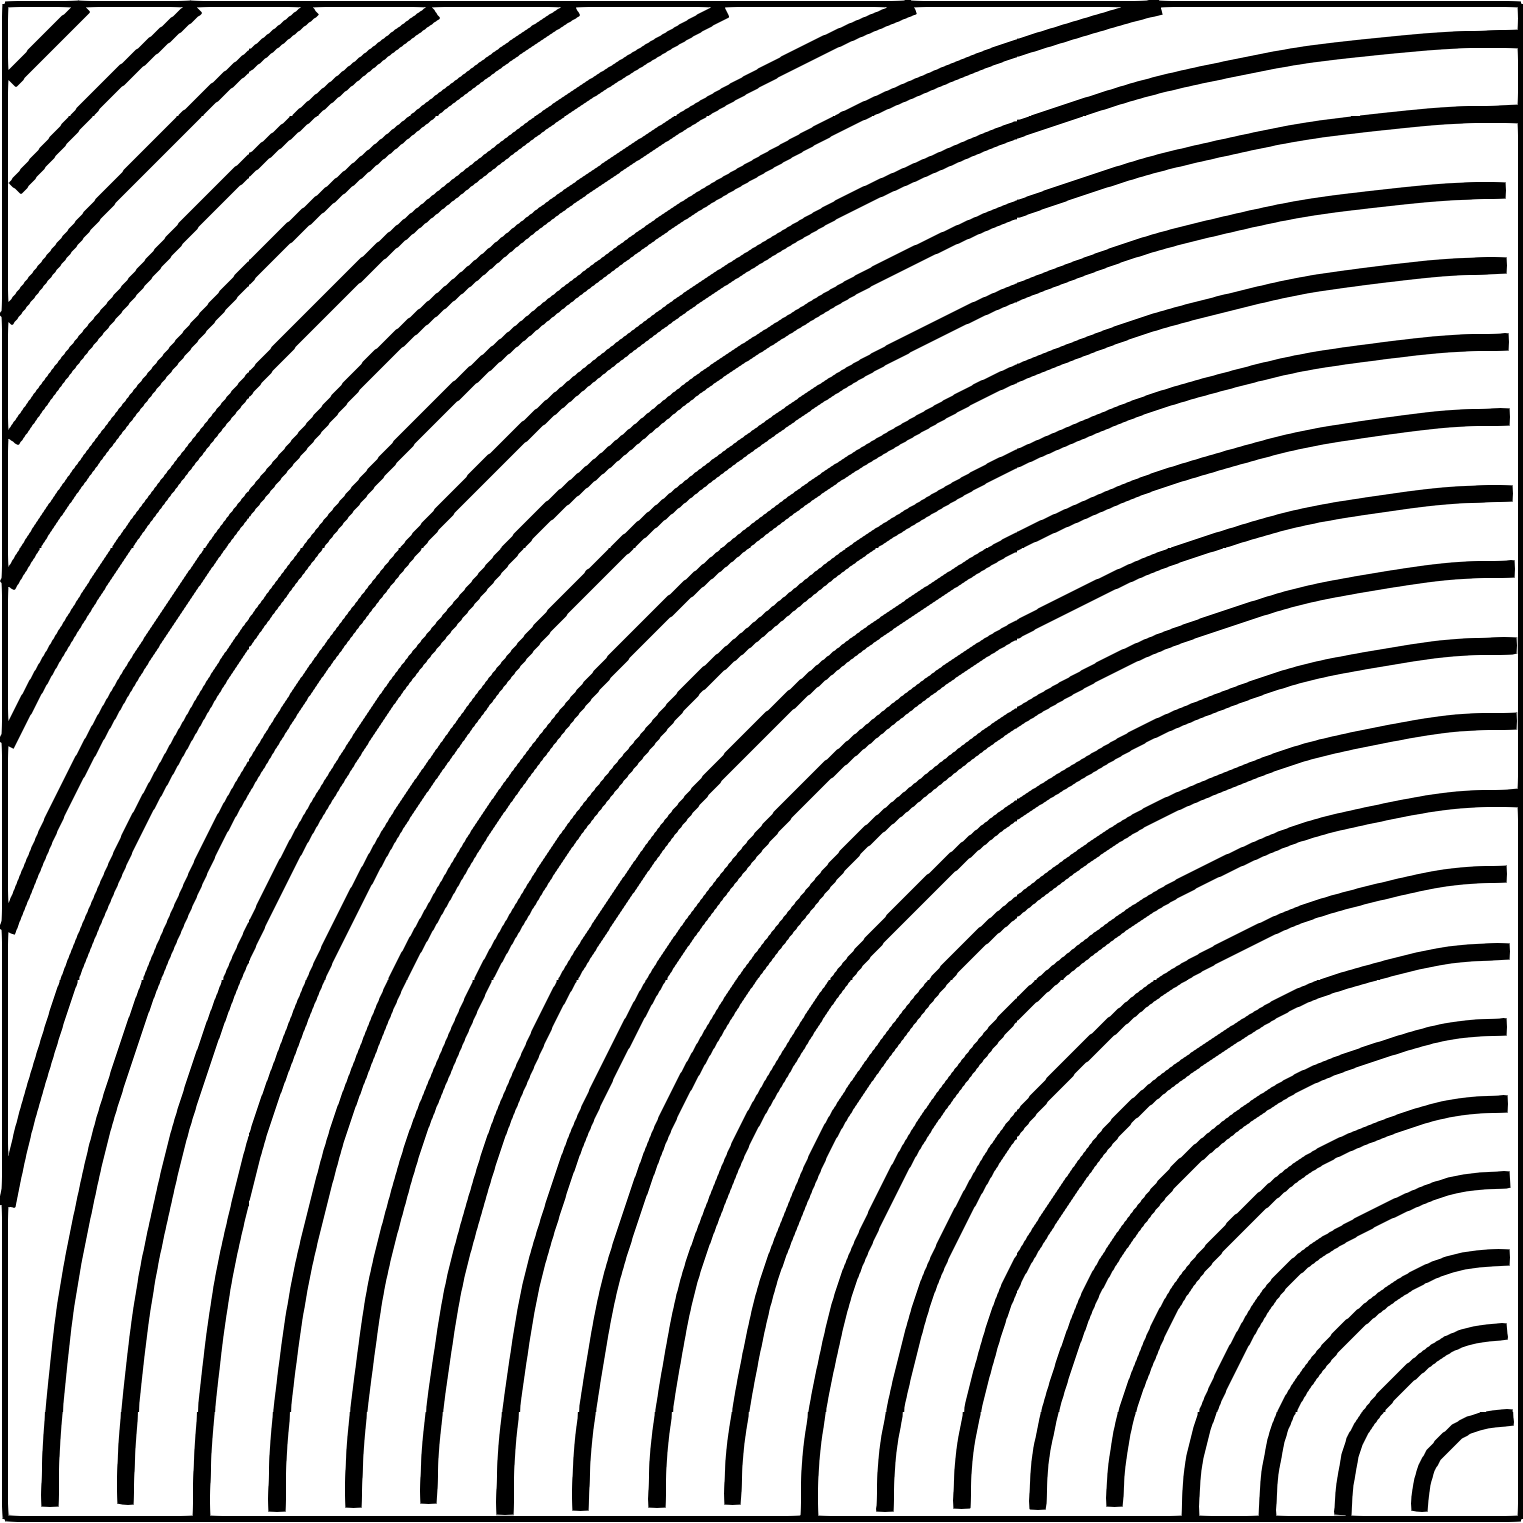
\includegraphics[scale=.1]{figures/OldAlgRotate.png}
        \caption*{(c)}
    \end{subfigure}
    \caption{
        (a) Forward and backward streamline integration through the field starting at the seed (red).
        The chosen sample points are drawn as a cross, and include the seed.
        (b) Equidistant seed candidates (green) obtained from the normals at the sample points are chosen for the next iteration.
        (c) Streamlines with equal distance generated by our algorithm in a field defined by $u(x,y)=(y, -x)^T$.}
    \label[figure]{fig:failedbasics}
\end{figure}
\vspace{-1cm}
\subsubsection{Streamline Traversal}
First, we choose a seed point from a list of candidates (initially an arbitrary point from the dataset)
and remove it from the list.
We then integrate forward and backward (\Cref{fig:failedbasics} (a)) to obtain the other points on the streamline,
until a given number of steps is reached, we leave the vector field's domain, or get too close to another streamline.
If the total length of the streamline is too short, we remove it.
To obtain the seed candidates, we compute the normals of the field at these points and add
points a distance $d_s$ away from them to the list (\Cref{fig:failedbasics} (b)).

\subsubsection{Seed Filtering}
The number of neighbor seed candidates is roughly 2$n$, where $n$
is the number of samples of the streamline we are integrating.
We use two filtering conditions to remove seeds that cannot produce a good streamline.
The first condition arises from roughly half the seeds generated by a streamline $L_1$ 
during the traversal process lying close to---if not precisely on---the preceding streamline, $L_0$,
because the seeds are placed a distance $d_s$ away, and the streamlines are mostly that same distance apart. 
The second condition is the distance to other seeds,
as starting a streamline from a seed that is too close to another will immediately end it.
Therefore, we filter two sets of seeds:
seeds generated during the traversal process and those present in the entire field.
\begin{figure}[ht]
    \centering
    \begin{subfigure}[b]{0.4\textwidth}
        \centering
        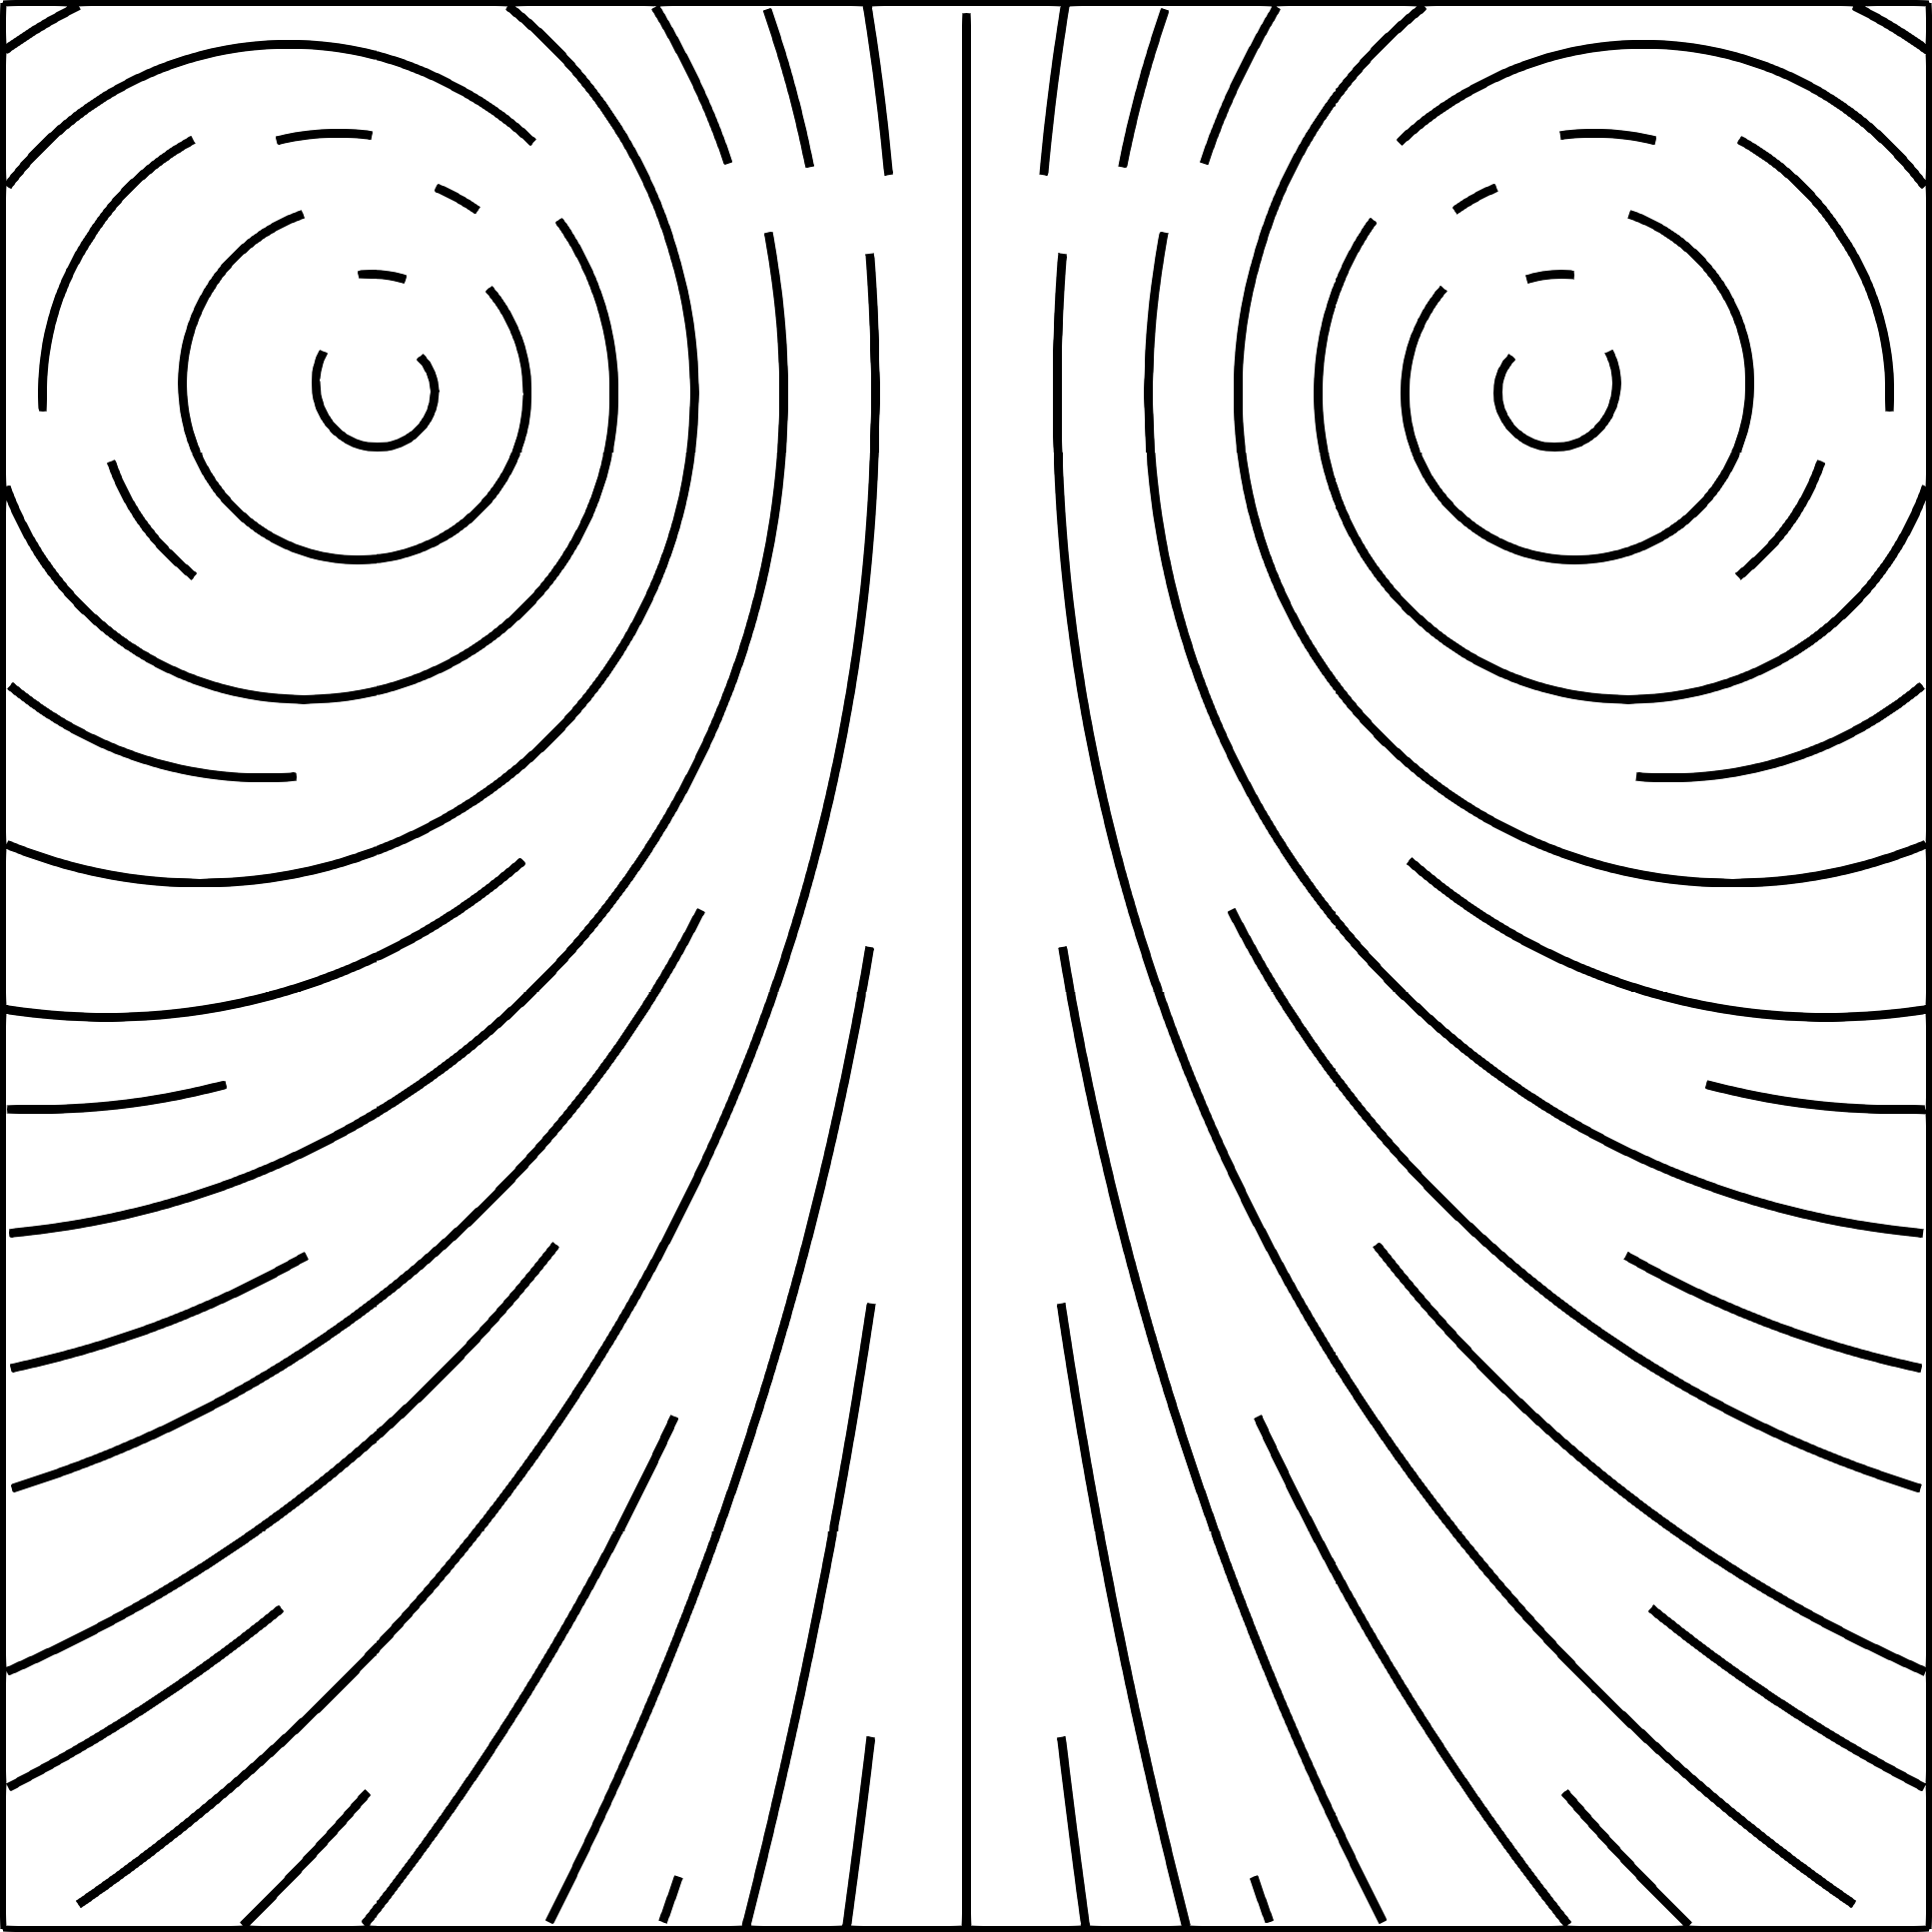
\includegraphics[scale=.1]{figures/OldAlgOrbit.png}
        \caption*{(a)}
    \end{subfigure}
    \begin{subfigure}[b]{0.4\textwidth}
        \centering
        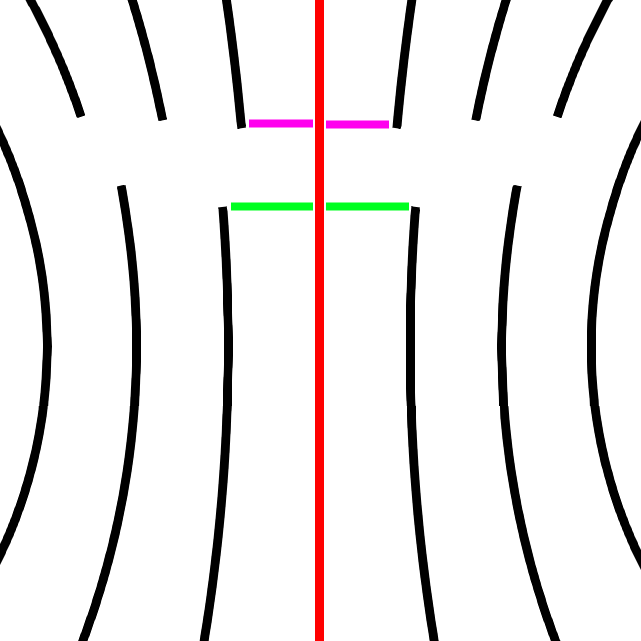
\includegraphics[scale=.3]{figures/OldAlgOrbitDistsZoom.png}
        \caption*{(b)}
    \end{subfigure}
    \caption{
        (a) Streamlines created in a double gyro dataset.
        (b) Top center zoom of (a). New streamlines created from the initial streamline (red) are cut off due to reaching $d_c$ (magenta).
        New streamlines are only drawn at distance grater than $d_c$,
        producing the gap between the upper and lower pairs of streamlines (black).
        The lower streamlines continue at a distance of $d_S$ (green).
    }
    \label[figure]{fig:cutoff}
\end{figure}
\subsubsection{Line Cutoff and Optimization}
To quickly filter the $2n$-pairs for points on the parent streamline,
we store the parent's points and remove any of the $2n$ seeds from the current step if they are too close.
When removing other seeds within range, we employ a grid with a spacing of $d_c$ and
use a dictionary to obtain lists of points inside the grid cell.
If we add a point during integration, we simply look up the coordinate and its eight
neighboring cells as a key to points in the area.
If we find a seed closer than $d_c$ in those cells, we remove it, allowing for an easy way to end
the integration when getting too close to another streamline (see \Cref{fig:cutoff}) as well:
We need only check whether we came close to another streamline's points during integration
(provided the integration step size is less than $d_c$, which is usually the case).

\newpage
\subsection{Steady Field Streamline Placement in 3D}
\label[section]{sec:3D}

\begin{figure}[ht]
    \centering
    \begin{subfigure}{.33\textwidth}
        \centering
        \setlength\pgfplotswidth{\textwidth}
        \begin{tikzpicture}
    \begin{axis}[ 
        ticks=none,
        axis lines = middle,
        axis line style={->},
        ymin=-.6, ymax=2.1,
        xmin=-.6, xmax=2.1,
        xlabel={$x$},
        ylabel={$z$},
        width=\pgfplotswidth,
        height=\pgfplotswidth
        ]
        \draw[rotate around={45:(.5,1)}] (axis cs:.5,1) ellipse (.6 and 1) [radius=1, fill=white];
        % Segment
        \draw[rotate around={45:(.5,1)}, ->, dotted, thick, red] (.5, 1) -- (1.5, 1) node[right] {$s$};
        % b0, b1
        \draw[rotate around={45:(.5,1)}, ->, blue!50] (.5, 1) -- (-.05, .85) node[right] {$b_0$};
        \draw[rotate around={45:(.5,1)}, ->, blue!50] (.5, 1) -- (.68, .09) node[right] {$b_1$};
      
        \draw[->] (0, 0) -- (-.5, -.5) node[right] {$y$};
    \end{axis}
\end{tikzpicture}

        \caption*{(a)}
    \end{subfigure}
    \begin{subfigure}{.33\textwidth}
        \centering
        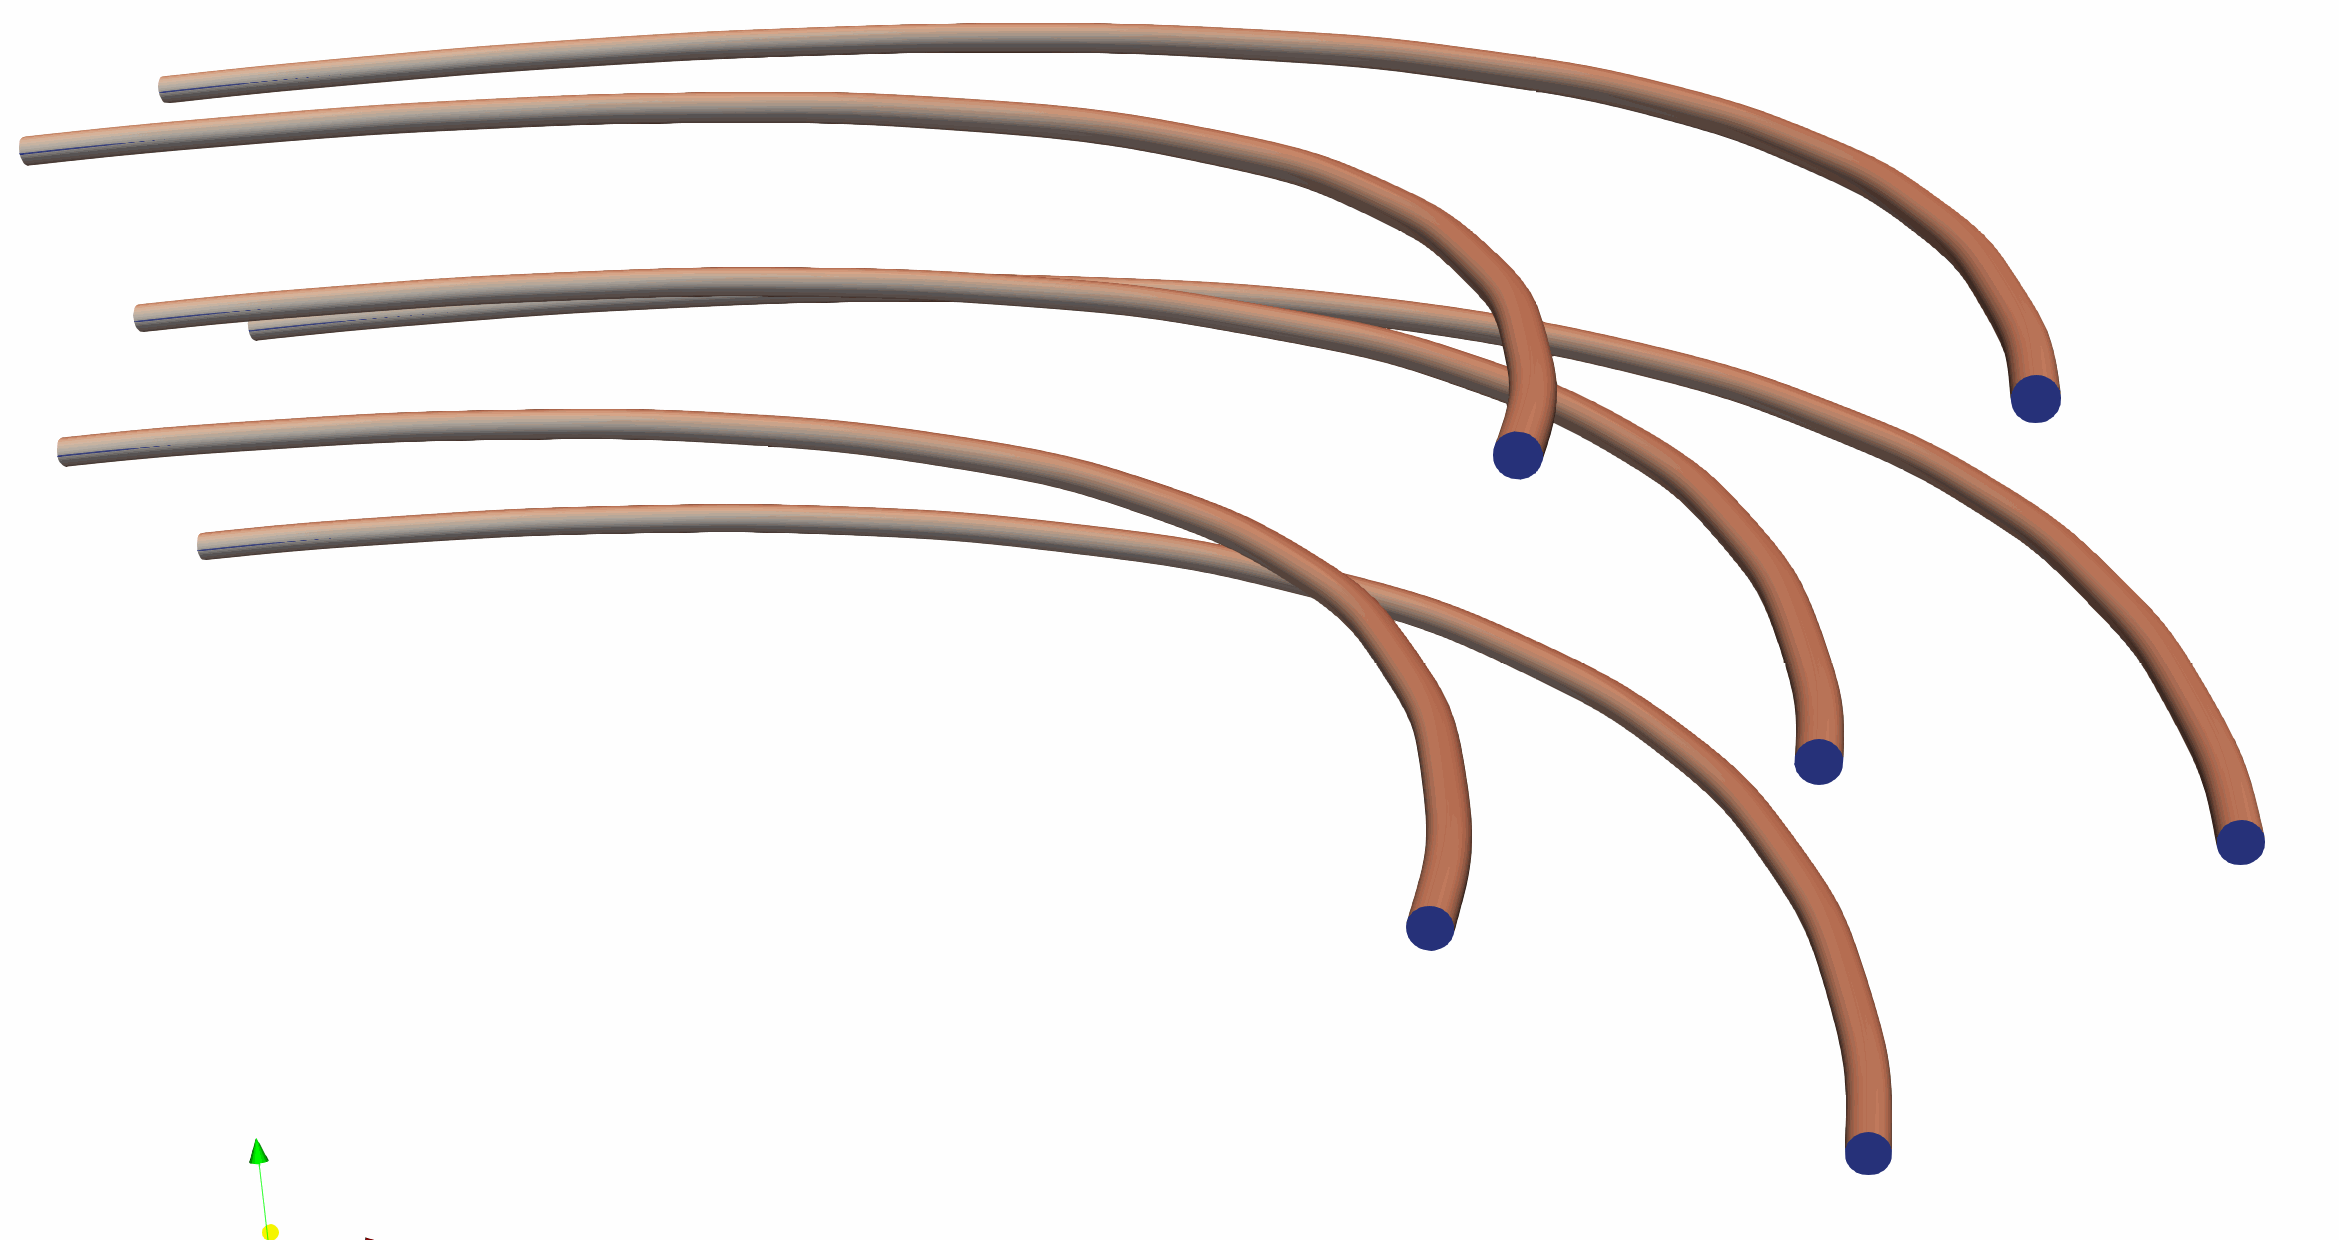
\includegraphics[scale=.05]{figures/OldAlg3D5.png}
        \vspace{5mm}
        \caption*{(b)}
    \end{subfigure}
    \begin{subfigure}{.3\textwidth}
        \centering
        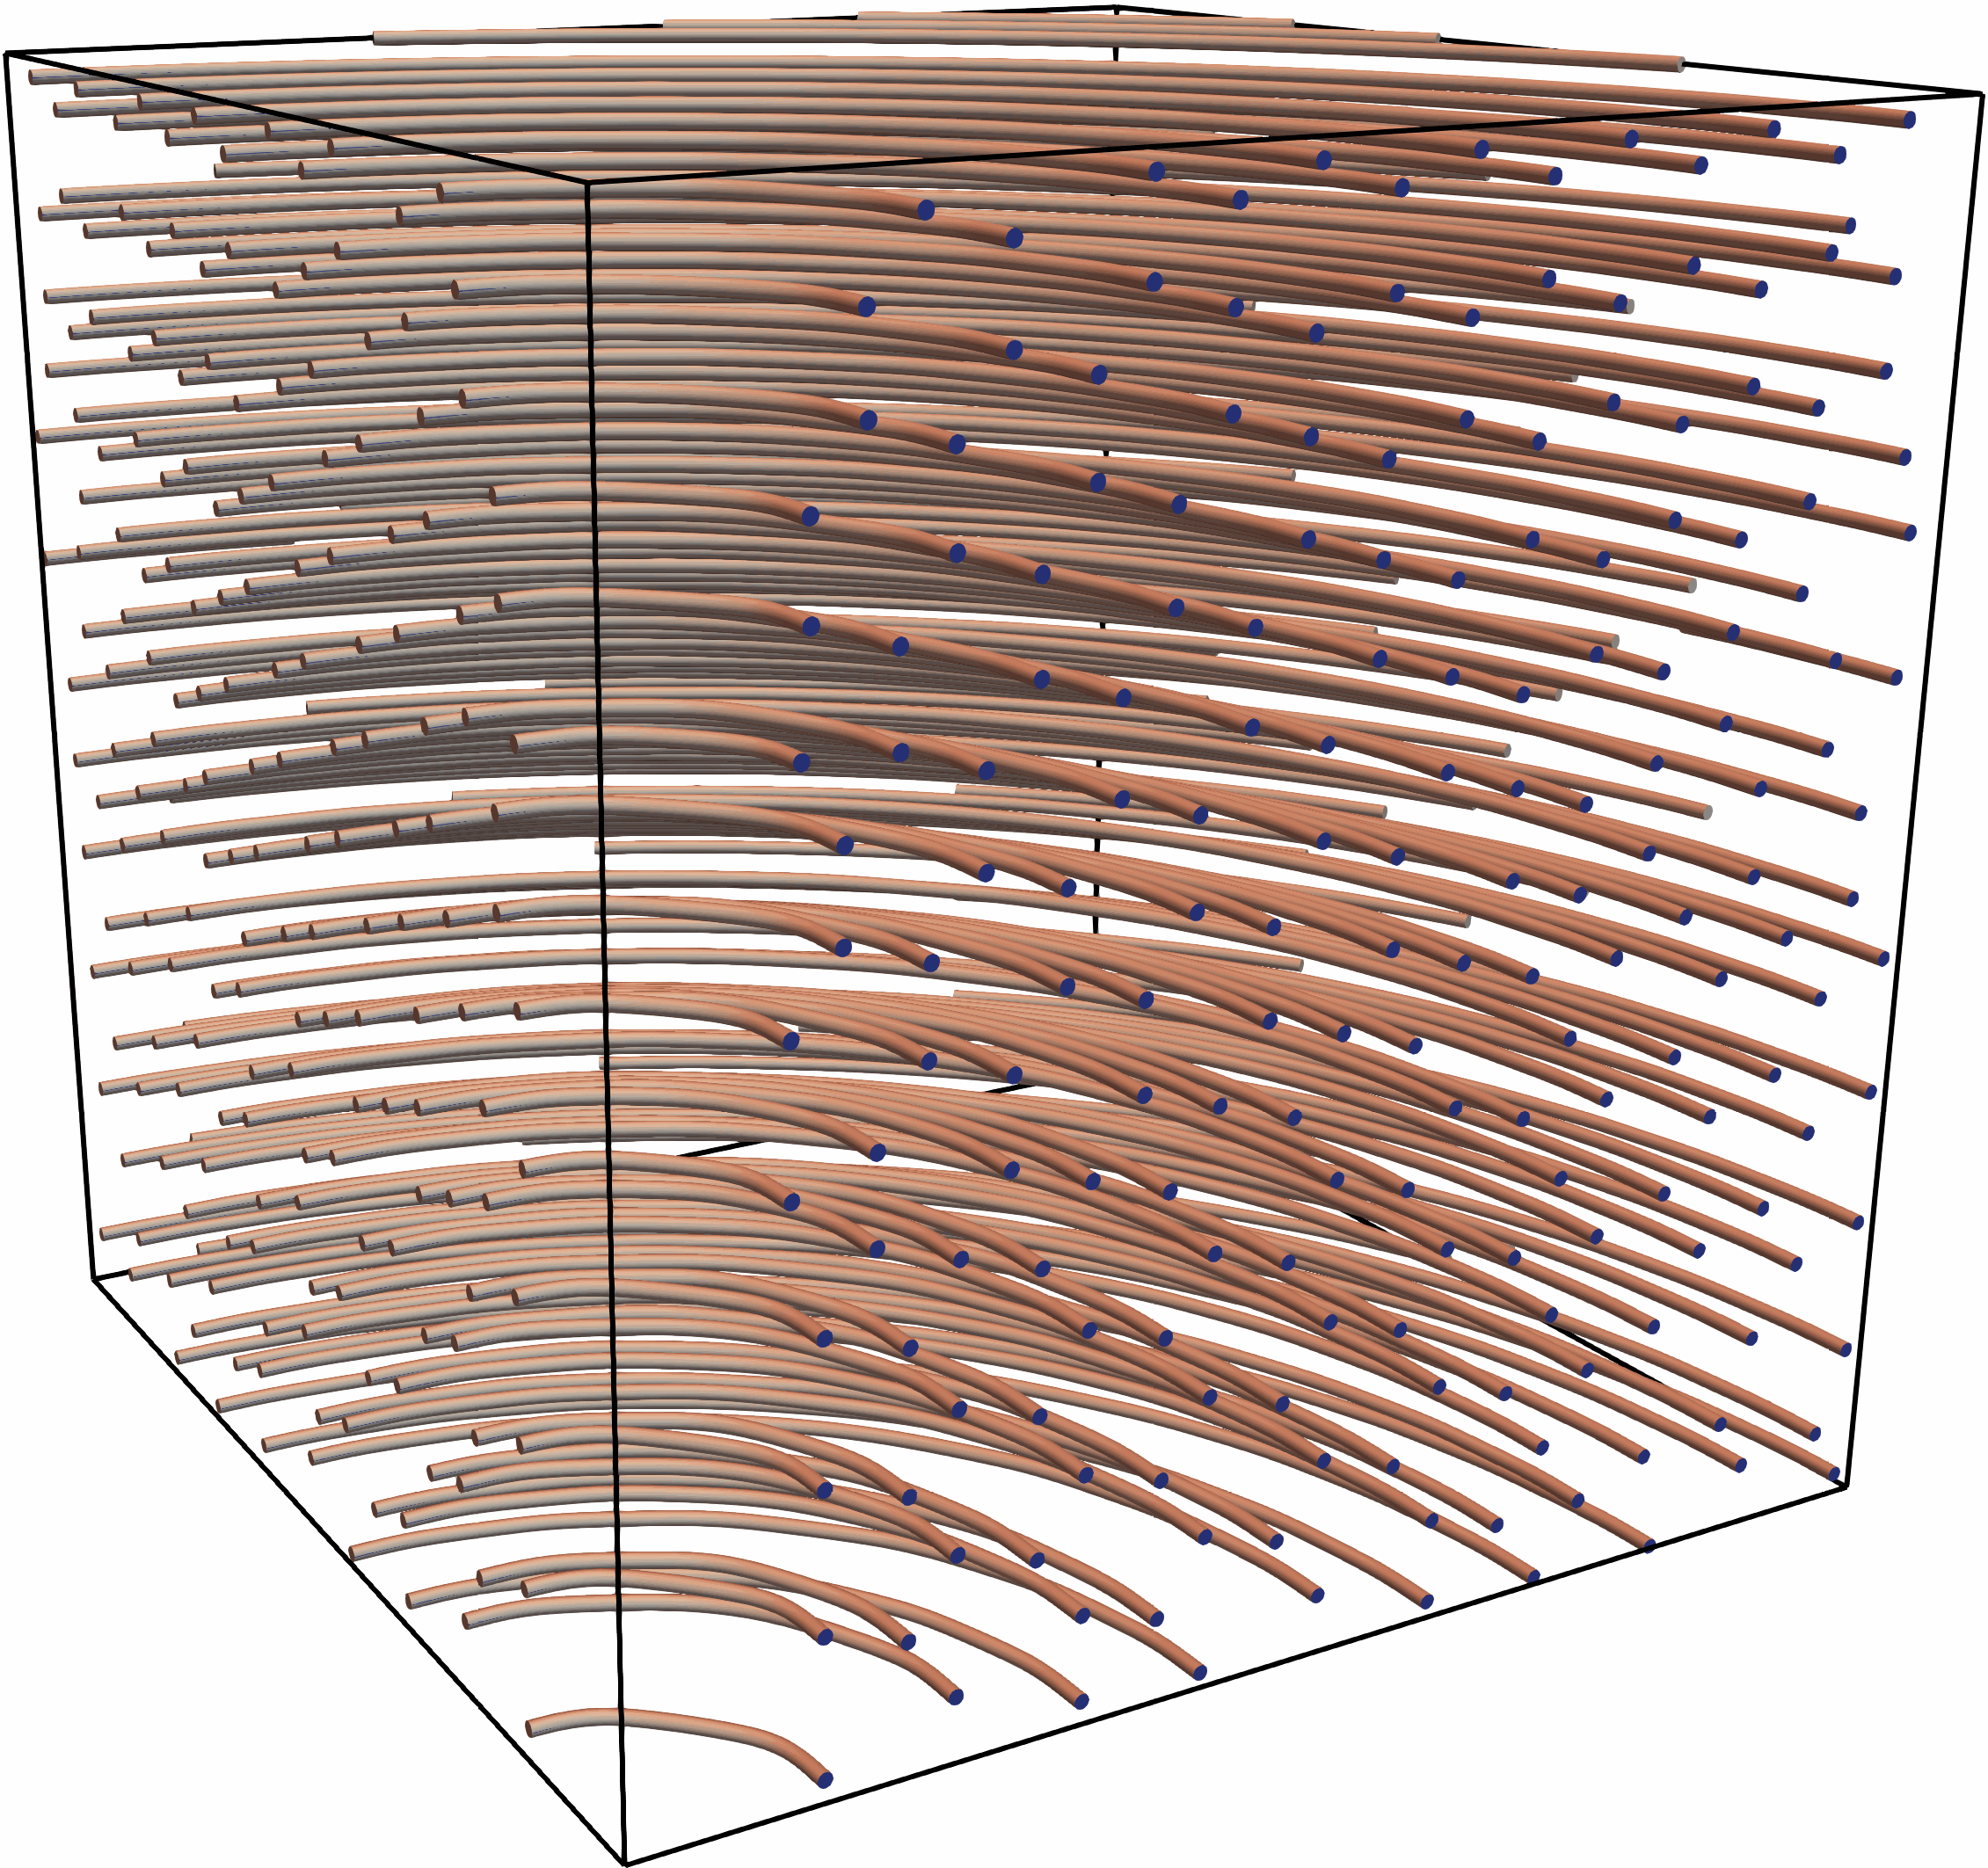
\includegraphics[scale=.05]{figures/OldAlg3D400.png}
        \caption*{(c)}
    \end{subfigure}
    \caption{
        (a) Normal plane of a streamline segment $s$ with two orthonormal basis vectors $\vectr{b}_0, \vectr{b}_1$.
        (b) Clear view of the center streamline with five neighbor streamlines evenly distributed at distance $d_S$.
        (c) Filled cube containing 254 streamlines. Notice the resemblance to \Cref{fig:failedbasics} (c).
    }
    \label[figure]{fig:failed3d}
\end{figure}
The most important part of generating streamlines in 3D is obtaining the seed locations.
In three dimensions, a vector has infinitely many normals, all lying on its normal plane.
Therefore, we define a number of points to evenly distribute around the streamline.
The process of obtaining these points is as follows.
Instead of the two trivial normals in 2D,
we now construct a normal plane around the streamline trajectory at the streamline's points.
For this, we find two vectors which are linearly independent of each other and the trajectory,
and then orthonormalize them to receive two orthonormal basis
vectors $\vectr{b}_0, \vectr{b}_1$ (see \Cref{fig:failed3d} (a)).
Having found $\vectr{b}_0$ and $\vectr{b}_1$, we can use the roots of unity as described in \Cref{sec:ROU} 
to obtain $k$ evenly spaced points on the complex unit circle $n_j\,,\; j=1, ..., k$.
Since the magnitude of $n_j$ is always one and $\vectr{b}_0, \vectr{b}_1$ are orthogonal,
we do a simple basis transformation into the 3D frame of reference.
We obtain the $j$-th 3D-vector $\vectr{v}_j$ from the $j$-th root using our basis vectors $\vectr{b}_0$ and $\vectr{b}_1$:
\[\vectr{v}_j = \operatorname{Re}(n_j)\cdot \vectr{b}_0 + \operatorname{Im}(n_j)\cdot \vectr{b}_1 \]
This gives us $k$ uniformly placed vectors on the normal plane around the current streamline segment.
The rest of the algorithm stays mostly the same as in 2D,
and the grid used for seed filtering is extended into the 3rd dimension accordingly.
See \Cref{fig:failed3d} (b, c) for an example using a 3D vector field.
\newpage
\subsubsection{Shortcomings}
\begin{figure}[ht]
    \begin{adjustwidth}{-2cm}{-2cm}
        \centering
        \begin{subfigure}[b]{.5\textwidth}
            \begin{overpic}[scale=.075, percent]{figures/OAH2D1.png}
                \put(0,0){\color{red}\linethickness{0.5mm}
                    \polygon(40,10)(55,10)(55,0)(40,0)
                    \polygon(33,45)(42,45)(42,15)(33,15)
                }
            \end{overpic}
            \caption{}
        \end{subfigure}
        \begin{subfigure}[b]{.5\textwidth}
            %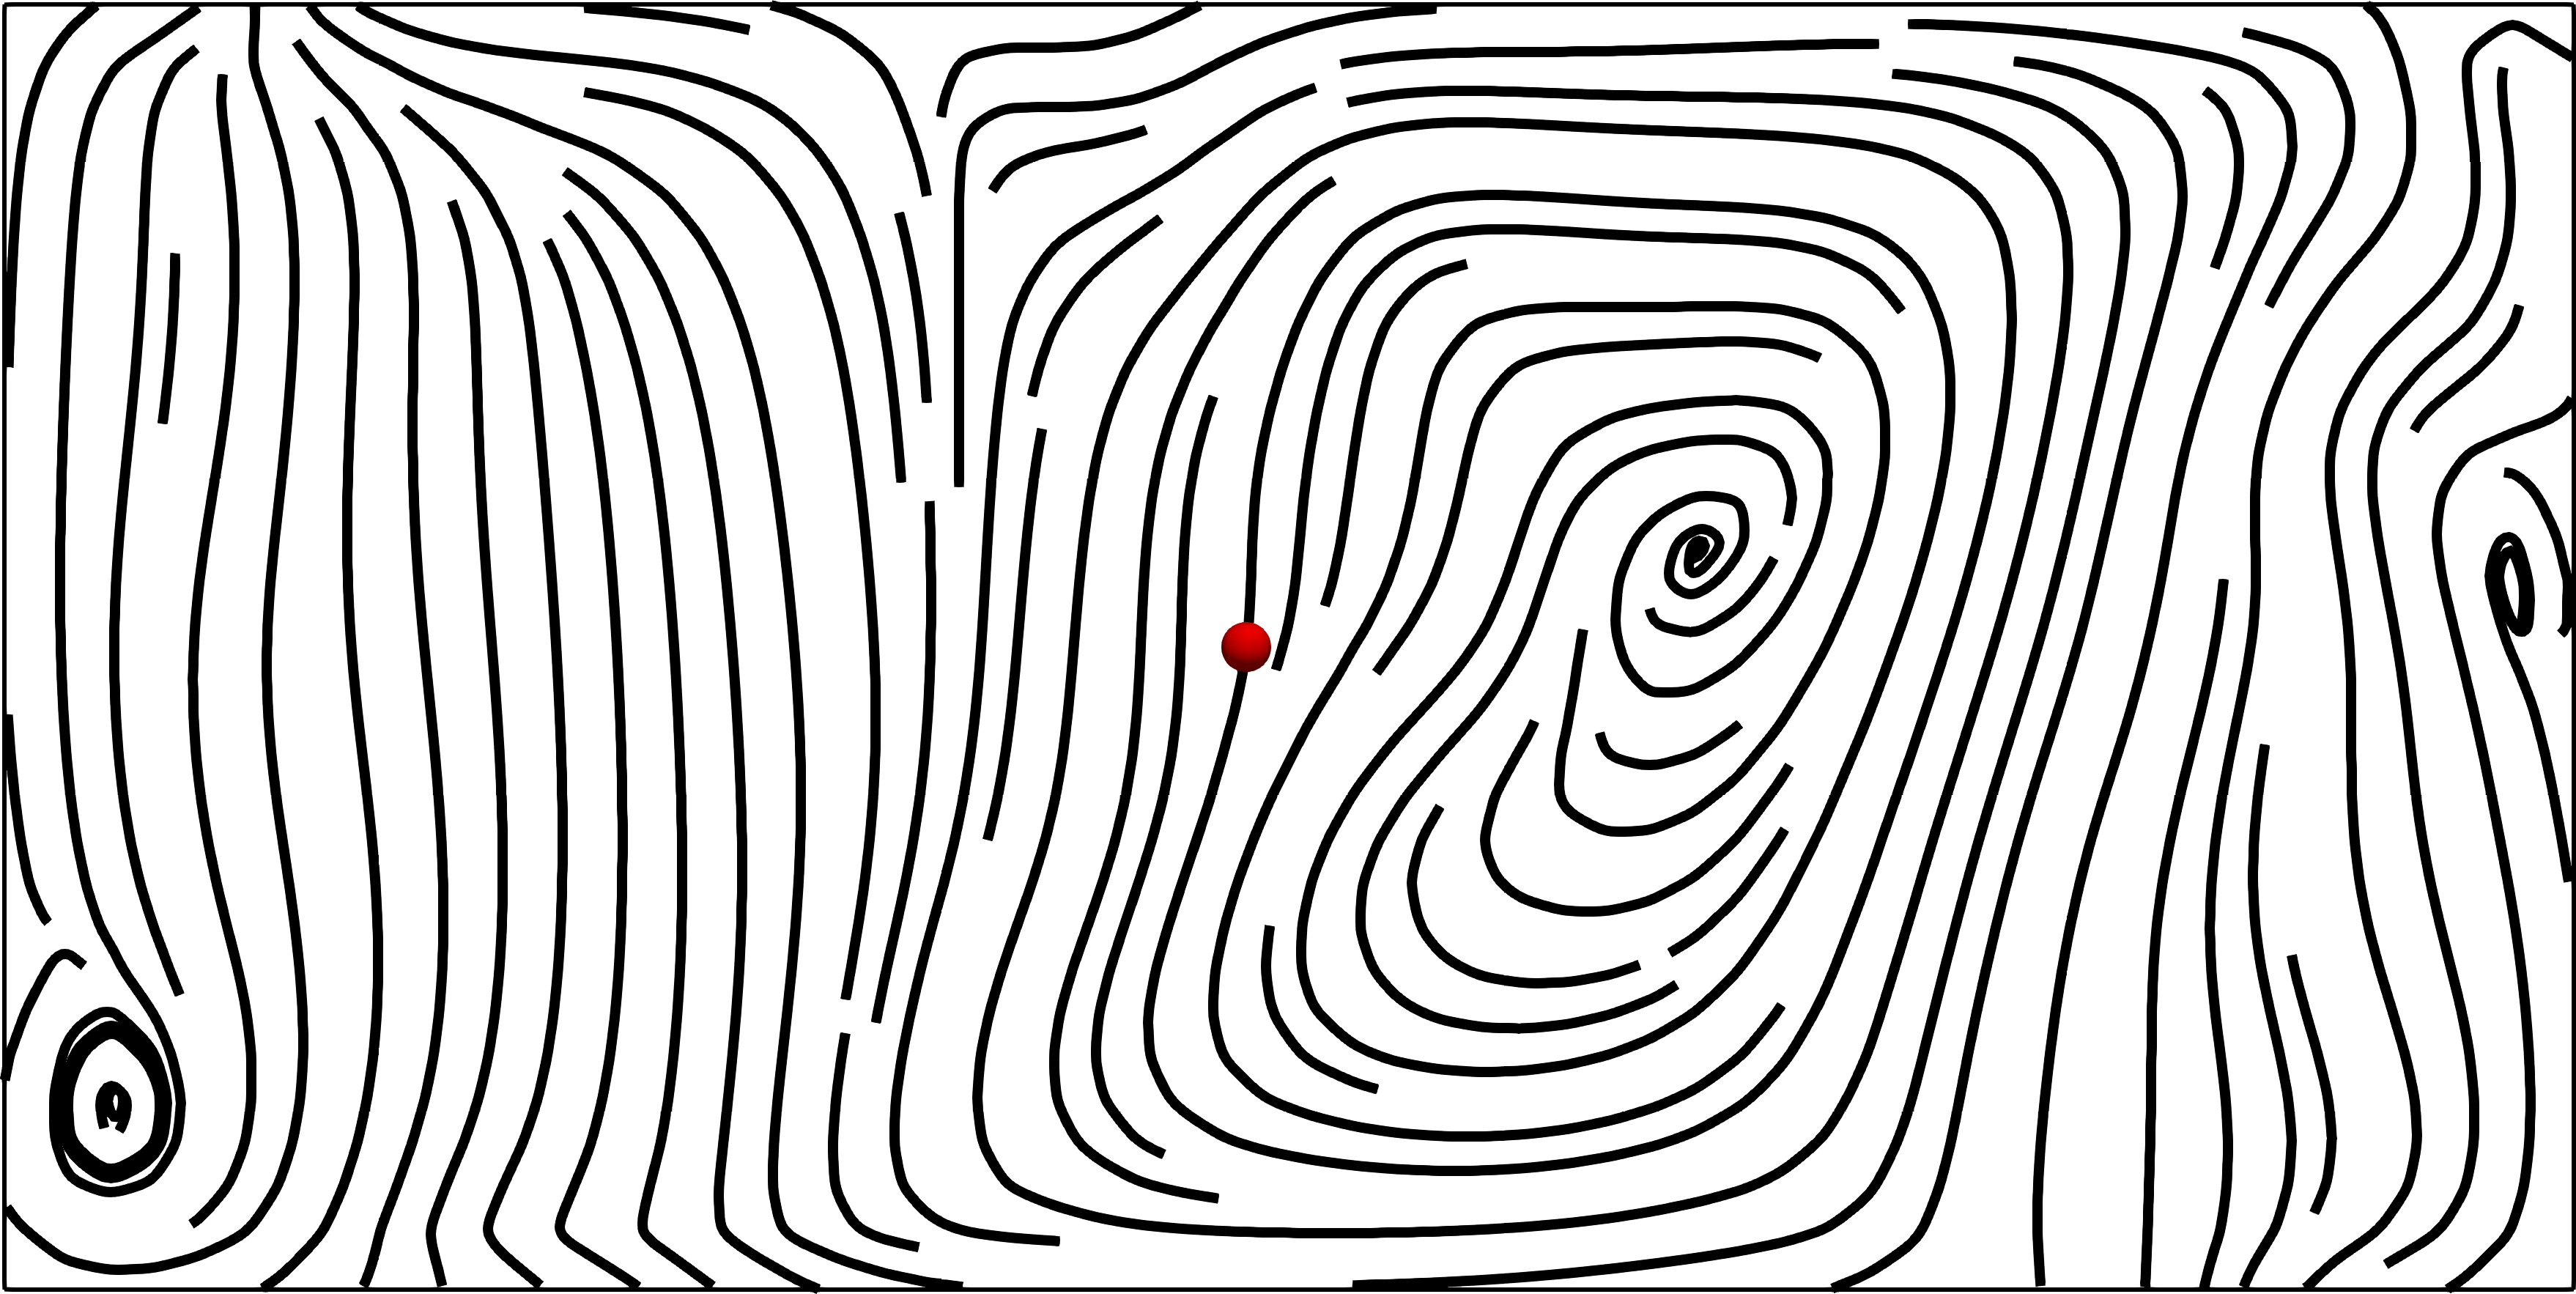
\includegraphics[scale=.075]{figures/OAH2D2.png}
            \begin{overpic}[scale=.075, percent]{figures/OAH2D2.png}
                \put(0,0){\color{blue}\linethickness{0.5mm}
                    \polygon(40,10)(55,10)(55,0)(40,0)
                    \polygon(33,45)(42,45)(42,15)(33,15)
                }
            \end{overpic}
            \caption{}
        \end{subfigure}
    \end{adjustwidth}
    \caption{
        Two different streamline placements for the same vector field.
        (a) hast its initial seed (red dot) directly at the center, (b)'s seed (blue dot) is moved by $0.01\,\%$ of image width,
        causing a completely different line image.
        The images look similar at first glance due to the density and rough shape being perceived the fastest
        by the human eye, but when following the individual lines the differences are easily noticeable.
        The stronger changes are indicated by the red and blue boxes,
        though differences visibly persist throughout most of the image.
    }
    \label[figure]{fig:failedshift}
\end{figure}
While this algorithm can quickly fill a space with streamlines according to the criteria mentioned above,
the main problem is the inability to react to small changes to streamlines,
which is primarily due to the strong hierarchical nature:
Since every streamline after the first comes from its predecessor,
a change at the ``root'' has drastic consequences for the succeeding streamlines (see \Cref{fig:failedshift}).
In the context of time coherence, the algorithm thus becomes unsustainable,
as an unsteady field is very likely to change at least slightly over the whole domain.
To make the streamlines time coherent,
we need to be able to move streamlines around without affecting the global scope too much in order
to compensate the small, field-induced streamline movements.
With this approach, changing the streamline's position after the generation of its neighbors
causes a re-evaluation of every streamline it is a predecessor of and leading to massive computational overhead.
Due to this problem, we do not see an effective way to implement time coherence with this approach,
and supersede it in favor of an image-guided one.
\newpage
